\section{Spektraleigenschaften von Graphen}

In diesem Kapitel wollen wir die in Abschnitt \ref{sss:ewgraph} behandelten Themen weiter vertiefen. Insbesondere werden wir einen Zusammenhang zwischen Krauszzerlegungen und den Eigenwerten eines Graphen herstellen. Da spezielle Krauszzerlegungen von Graphen (n"amlich diejenigen mit Minimalgrad mindestens $2$) in Zusammenhang mit Vermutung \ref{con:efl} stehen, werden wir hier eine alternative Herangehensweise an die Vermutung finden. 

\subsection{Krauszzerlegungen und Eigenwerte}
\begin{theorem}
  \label{thm:KrauszEigenwerte}
  Seien $G$ ein Graph mit $V(G)=\{v_1,\dots,v_n\}$ und $\mathcal K=\{K^1,\dots,K^p\}$ eine Krauszzerlegung von $G$ mit $\delta(\mathcal K) \geq d \geq 2$ . Desweiteren sei $d_i = d_{\mathcal{K}}(v_{i})$ f"ur $1\leq i \leq n$. 
  Dabei w"ahlen wir die Eckennummerierung so, dass $d_1 \geq \dots \geq d_{n}$ ist.
  Dann gelten folgende Aussagen : 
  \begin{enumerate}[label=\rm{(\alph*)}]
    \item $\lambda_i(G) \geq -d_{n-i+1}$ f"ur $i = 1, \dots , n$.
    \item $\lambda_{p+1}(G) \leq -d$ falls $p < n$ ist.
  \end{enumerate}
\end{theorem}

\begin{proof}
  Zun"achst zeigen wir (a). Es sei $A=A(G)$ die Adjazenzmatrix von $G$ und $D = \operatorname{diag}(d_1,\dots,d_n)$. Definiere $B\in\R^{n\times m}$ als die Inzidenzmatrix von $\mathcal K$, also $$B_{ij} = \begin{cases}
    1 & \text{falls } v_i \in K^j \\ 0 & \text{falls }v_i \notin K^j
  \end{cases}$$ 
  Nun betrachten wir $M=BB^{T}$. Es gilt
  \[
    M_{ij} = \sum\limits_{k=1}^{m}B_{ik}B^{T}_{kj} = \sum\limits_{k=1}^{m}B_{ik}B_{jk}
  \]
  Seien $1\leq i < j \leq n$. Da $B$ die Inzidenzmatrix von $\mathcal{K}$ ist, gilt  $$ B_{ik} B_{jk} = 1 \Leftrightarrow B_{ik} = 1 \text{ und } B_{jk} = 1 \Leftrightarrow v_i,v_j \in K^{k}.$$ Ist $v_iv_j \in E(G)$, so kommt die Kante $v_iv_j$ in genau einem $K\in \mathcal{K}$ vor, d.h. es gibt genau ein $k\in \left\{ 1,\dots,m \right\}$ f"ur das $B_{ik}$ und $B_{jk}$ gleich $1$ sind. Ist $v_iv_j\notin E(G)$, so kommt die Kante $v_iv_j$ auch nicht in einem der Graphen der Krauszzerlegung vor.
  Also ist f"ur alle $k\in \left\{ 1,\dots, m \right\}$ $B_{ik}B_{jk} = 0$. Folglich ist $M_{ij}=1$ genau dann, wenn $v_iv_j\in G$. Also ist $M_{ij} = A_{ij}$.
  Sei nun $1\leq i \leq n$. Dann gilt f"ur die Diagaonaleintr"age $M_{ii}$ der Matrix $M$:
  \[
    M_{ii} = \sum\limits_{k=1}^{d}B_{ik}B_{ik} = \sum\limits_{k=1}^{d} B_{ik}.
  \]
  Die Gleichung $B_{ik}=1$ ist genau dann erf"ullt, wenn $v_i \in K^k$. Folglich ist $M_{ii}= d_{\mathcal{K}}(v_i)= d_i$. Damit gilt $M=A+D$. Au{\ss}erdem ist die Matrix $M=BB^{T}$ nach Satz \ref{prop:psdmatrix} positiv semidefinit.
  Folglich ist $A- (-D)$ positiv semidefinit und es folgt mit Lemma \ref{lem:evpsddif}, dass 
  \begin{equation*}
    \lambda_i(G) = \lambda_i(A) \geq \lambda_i(-D) = -d_{n-i+1}
  \end{equation*}
  Damit ist (a) gezeigt.

  Nun zeigen wir (b). Sei $p<n$. Dann ist $\operatorname{rang}(M)= \operatorname{rang}(B) \leq p$. Also ist $\lambda_{p+1}(M) = 0$ und es folgt mit Satz \ref{thm:weylineq}, dass 
  \begin{align*}
    \lambda_{p+1}(A) + d \leq \lambda_{p+1}(A) + d_{n} = \lambda_{p+1}(A) + \lambda_{n} (D) \leq \lambda_{p+1} (M) = 0
  \end{align*}
  Durch Umstellen erhalten wir die gew"unschte Ungleichung.
\end{proof}

Wir wollen nun eine Folge von Graphenparametern definieren. Seien dazu $d\geq 1$ und $G$ ein Graph. Wir bezeichnen mit $\xi_{d}(G)$ die Anzahl aller Eigenwerte von $G$, welche echt gr"o{\ss}er als $-d$ sind. Damit ist also 
$$\xi_{d}(G) = |\set{i}{\lambda_i(G) > -d}|.$$
Dieser ist ein Graphenparamter, da nach Lemma \ref{lem:GraphEigenwerte} isomorphe Graphen das selbe Spektrum besitzen und somit $\xi_d $ zwei isomorphen Graphen die selbe nat"urliche Zahl zuordnet. 

\begin{lemma}
  Seien $G$ ein Graph und $d\in \N$. Dann gelten f"ur den Graphenparameter $\xi_d$ folgende Aussagen:
  \begin{enumerate}[label={\rm(\alph*)}]
    \item Ist $H$ ein induzierter Untergraph von $G$, so gilt $\xi_{d}(H) \leq \xi_{d}(G)$.
    \item Ist $d\geq 2$, so gilt $\omega(G) \leq \xi_{d}(G)$.
    \item $\alpha(G) \leq \xi_{d}(G)$. 
    \item Ist $v\in V(G)$ eine Ecke von $G$, so gilt $\xi_{d}(G) \leq \xi_{d}(G-v) +1$.
    \item Ist $d'\in\N$ mit $d \leq d'$, so gilt $\xi_{d}(G) \leq \xi_{d'}(G)$.
  \end{enumerate}
  \label{lem:xieigenschaften}
\end{lemma}

\begin{proof}
  Wir zeigen zun"achst (a). Sei $\xi_{d}(H) = l$. Folglich ist $\lambda_{l}(H) > -d$ und wir erhalten mit Lemma \ref{lem:InterlacingGraphen}, dass $\lambda_{l}(G) \geq \lambda_{l}(H) > -d$ gilt. Deswegen ist $\xi_{d}(G) \geq l = \xi_{d}(H)$. Also gilt (a).

  Um (b) und (c) zu zeigen, seien $p = \omega(G)$ und $q=\alpha(G)$. Nach Korollar \ref{cor:alphaomegaEigenwerte} ist dann $\lambda_{p}(G) \geq -1$ und $\lambda_q(G) \geq 0$ und deswegen $\xi_{d}(G) \geq p = \omega(G)$ f"ur $d \geq 2$ und $\xi_{d}(G) \geq q = \alpha(G)$ f"ur alle $d \in \N$. 

  F"ur den Beweis von (d) w"ahlen wir eine beliebige Ecke $v\in V(G)$ von $G$. Dann ist $G-v$ ein induzierter Untergraph von $G$ der Ordnung $|G|-1$. Sei $l=\xi_{d}(G-v)$. Ist $l= |G|-1$, so ist nichts zu zeigen, da $\xi_d(G)$ nach oben durch $|G|$ beschr"ankt ist. Andernfalls ist $l< |G| -1$. 
  Dann ist $\lambda_{l}(G-v) > -d$ und $\lambda_{l+1}(G-v) \leq -d$. Nun folgt mit Lemma \ref{lem:InterlacingGraphen}, dass $$\lambda_{l+2}(G) \leq \lambda_{l+1}(G-v) \leq -d$$ richtig ist. Deswegen ist $\xi_{d}(G) \leq l+1 = \xi_{d}(G-v) +1$. 

  Aussage (e) gilt, da die Eigenwerte eines Graphen fallend geordnet sind.
\end{proof}

Mit Satz \ref{thm:KrauszEigenwerte} erhalten wir sofort Aussagen "uber Krauszzerlegungen von $G$, falls $G$ bestimmte Untergraphen enth"alt.
\begin{corollary}
  \label{cor:Korollar1}
  Seien $G$ ein Graph und $H$ ein induzierter Untergraph von $G$. Desweiteren seien $q,d \in \N$ mit $\xi_{d}(H) \geq q$. Dann ist $\kappa_{d}(G) \geq q$.
\end{corollary}

\begin{proof}
  Da $H$ ein induzierter Untergraph von $G$ ist, folgt aus Lemma \ref{lem:xieigenschaften}, dass $\xi_{d}(G) \geq q$ gilt. Also ist $\lambda_{q}(G) > -d$. 
  Angenommen, es gilt $p = \kappa_{d}(G) < q$. Dann gibt es  eine Krauszzerlegung $\mathcal{K}$ von $G$ mit $|\mathcal{K}| = p$ und $\delta(\mathcal{K}) \geq d$. Aus Satz \ref{thm:KrauszEigenwerte} folgt, dass $\lambda_{q}(G) \leq \lambda_{p+1}(G) \leq -d $ gilt. Dann ist aber auch $\xi_{d}(G) < q$ und wir erhalten einen Widerspruch. Folglich ist $\kappa_2(G) \geq q$.
\end{proof}

\begin{corollary}
  \label{cor:LineGraphWald}
  Seien $G$ ein Graph und $H$ ein induzierter Untergraph von $G$. Ist $H$ Kantengraph eines Waldes, so gilt 
  $\kappa_{2}(G)\geq \left|H\right|$.
\end{corollary}

\begin{proof}
  Ist $\delta(G) \leq 1$, so ist nichts zu zeigen, da dann mit \ref{lm:krauszexistenz} folgt, dass $\kappa_2(G) = \infty$ richtig ist.

  Sei sonst $q = |H|$. Da $H$ Kantengraph eines Waldes ist, folgt $\lambda_{q}(H) > -2$ aus Korollar \ref{cor:linegraphwald}. Also ist $\xi_{2}(H) = |H|$.
  Dann ist mit Korollar \ref{cor:Korollar1} $\kappa_{2}\left( G \right) \geq \left| H\right|$.
\end{proof}
Der folgende Korollar wurde bereits von Klotz \cite{Klotz89} gezeigt. Wir erhalten "uber die Krauszzerlegung und Korollar \ref{cor:LineGraphWald} jedoch einen eleganten Beweis.
\begin{corollary}[Klotz]
  $\kappa_{2}\left( K_n \right) \geq n$
\end{corollary}

\begin{proof}
  $K_n$ ist der Kantengraph von $K_{1,n}$. Nun folgt die Behauptung aus Korollar \ref{cor:LineGraphWald}.

  Einen zweiten Beweis erhalten wir durch Betrachten der Eigenwerte von $K_n$. Nach Lemma \ref{lem:xieigenschaften} gilt $n = \omega(K_n) \leq \xi_{2}(K_n)$. Somit folgt die Behauptung aus Korollar \ref{cor:Korollar1}.
\end{proof}

\begin{corollary}
  Ist $G$ ein Graph so gilt $\omega\left( G \right)\leq \kappa_{2}\left( G \right)$ und $\alpha\left( G \right)\leq \kappa_{2}\left( G \right)$.
  \label{cor:alphaomegakrausz}
\end{corollary}

\begin{proof}
  Aus Lemma \ref{lem:xieigenschaften} folgt
  \begin{align*}
    \omega(G) &\leq \xi_{2}(G) \leq \kappa_{2}(G) \\
    \alpha(G) &\leq \xi_{2}(G) \leq \kappa_{2}(G) 
  \end{align*}
  und damit die Behauptung.
\end{proof}

Um die Erd\H{o}s--Faber--Lov\'asz Vermutung zu beweisen, gen"ugt es zu zeigen, dass jeder Graph $G$ die Ungleichung $$\chi(G) \leq \xi_{2}(G)$$ erf"ullt. Dann gilt mit Korollar \ref{cor:Korollar1} $$\chi(G) \leq \kappa_{2}(G),$$  woraus mit Satz \ref{thm:MainTheorem} dann Vermutung \ref{con:efl} folgt.

Eine M"oglichkeit dies zu zeigen, w"are zu beweisen, dass $\xi_2$ ein Szekeres-Wilf-Paramter ist. Die Eigenschaft (S1) ist nach den obigen "Uberlgungen erf"ullt. Berechnungen in Maple zeigen jedoch, dass Eigenschaft (S2) nicht immer erf"ullt ist. 

Es ist jedoch m"oglich die chromatische Zahl durch eine Funktion von $\xi_2$ nach oben zu beschr"anken, wie der folgende Satz zeigt. Dazu ben"otigen wir einen weiteren Parameter, $\beta$, welcher f"ur einen Graphen $G$ wie folgt definiert ist:
$$\beta(G) = \max\set{|H|}{H\unlhd G, \lambda_{min}(H) > -2}.$$

\begin{lemma}
  Ist $G$ ein Graph mit $\beta(G) \leq p$ und $\omega(G) \leq q$, so existiert eine Funktion $f:\N ^{2} \to \N$ f"ur die $\chi(G) \leq f(p,q) $ gilt. 
  \label{lem:funktionxilemma}
\end{lemma}
\begin{proof}
  Wir beweisen die Aussage durch Induktion nach $\omega(G)$. Sei also $\beta(G) \leq p$ f"ur $p\in \N$. Ist $\omega(G) \leq 1$, so ist $\chi(G) \leq 1$ und wir k"onnen $f(p,1) = 1$ w"ahlen.

  Sei nun $\omega(G) \leq q$ mit $q \geq 2$ und gelte f"ur alle Graphen $H$ mit $\omega(H) \leq q-1$, dass $\chi(H) \leq f(p,q-1)$ f"ur alle $p \in \N$ erf"ullt ist.
  Ist $\omega(G) \leq q-1$, so folgt die Aussage durch die Induktionsvoraussetzung. Andernfalls ist $\omega(G) = q$ und $\beta(G) = l \leq p$. Dann gibt es einen induzierten Untergraphen $H$ von $G$, sodass $|H|=l$ und $\lambda_{min}(H)> -2$. F"ur $v\in V(H)$ sei $N_v = \set{u\in V(G)}{uv\in E(G)}$, die Menge der Nachbarn von
  $v$ in $G$. Dann ist $\omega(G[N_v]) \leq \omega(G) -1 $, da sonst $G[N_v\cup \{v\}]$ einen vollst"andiger Graphen der Ordnung $p+1$ enth"alt, was nicht m"oglich ist, da $\omega(G) \leq p$ ist. Au{\ss}erdem gilt $\beta(G[N_v]) \leq \beta(G)$, da jeder induzierte Untergraph von $G[N_v]$ wieder ein induzierter Untergraph von $G$ ist. Wegen der Induktionsvorraussetzung folgt dann, dass $\chi(G[N_v]) \leq f(p,q-1)$ richtig ist. 
  Wir w"ahlen $$N = V(G) \setminus \bigcup\limits_{v\in V(H)} N_v,$$ die Menge aller Ecken von $G$ die mit keiner Ecke von $H$ benachbart sind. Wir zeigen, dass $G[N]$ kantenlos ist. W"are dem nicht so, so existiert eine Kante $uv\in E(G[N])$. 
  Dann kommen beide Ecken nach Definition von $N$ nicht in $V(H)$ vor. 
  Also gilt $u,v\notin V(H)$ und weder $u$ noch $v$ ist mit einer Ecke aus $H$ benachbart. Wir betrachten den Graphen $$H' = G[V(H) \cup \{u,v\}].$$ Dieser ist ebenfalls ein induzierter Untergraph von $G$ mit $|H'| > |H|$. Da er die disjunkte Vereinigung von $H$ und einem vollst"andigen Graphen der Ordnung $2$ ist, ist das Spektrum von $H'$ die Vereinigung des Spektrums von $H$ und $(1,-1)$. Insbesondere ist $$\lambda_{min}(H') = \min \{\lambda_{min}(H), -1\} > -2.$$ 
  Dies ist ein Widerspruch zur Wahl von $H$. Also ist $G[N]$ kantenlos und folglich gilt $\chi(G[N]) \leq 1$. 
  Wegen der Subadditivit"at der chromatischen Zahl und $|H| \leq \beta(G) \leq q$ gilt dann $$\chi(G) \leq \chi(G[N]) + \sum\limits_{v\in V(H)}\chi(G[N_v]) \leq 1 + |H|f(p,q-1)  \leq 1+p\cdot f(p,q-1).$$

  Also folgt aus dem Prinzip der vollst"andigen Induktion, dass die Funktion $f$ eine obere Schranke f"ur $\chi(G)$ ist.
\end{proof}
Mit dieser Vorarbeit k"onnen wir nun den folgenden Satz beweisen.
\begin{theorem}
  Es gibt eine Funktion $g:\N \to \N$ welche $$\chi(G) \leq g(\xi_{2}(G))$$ f"ur alle Graphen $G$ erf"ullt. 
  \label{thm:funktionxi}
\end{theorem}

\begin{proof}
  Wir zeigen, dass f"ur alle Graphen $G$ die Ungleichung $\beta(G) \leq \xi_{2}(G) $ erf"ullt ist. Dann folgt die Behauptung, indem wir $g(\xi_2(G))=f(\xi_2(G),\xi_2(G))$ setzen, wobei $f$ die Funktion aus \ref{lem:funktionxilemma} ist.

  Sei also $\beta(G) = l \in \N$. Dann existiert ein induzierter Untergraph $H$ von $G$ mit $|H| = l$ und $\lambda_{min}(H) = \lambda_{l}(H) > -2$. Folglich ist mit Lemma \ref{lem:InterlacingGraphen} $\lambda_l (G) \geq \lambda_{l}(H) > -2$, was $\xi_2(G) \geq l = \beta(G)$ impliziert.
\end{proof}

\begin{theorem}
  \label{thm:MainTheorem}
  Existiert ein $d\in \N$, sodass f"ur alle  Graphen $G$ $$\chi(G) \leq \xi_{d}(G)$$ gilt, so gelten die folgende Aussagen:
  \begin{enumerate}[label=\rm{(\alph*)}]
    \item F"ur alle Graphen $G$ gilt $\chi(G) \leq \kappa_d (G)$.
    \item  Ist $H$ ein linearer Hypergraph mit $\left|e\right| \geq d$ f"ur alle $e\in E(H)$, so ist $\chi'\left( H \right)\leq \left|H\right| $
  \end{enumerate}
\end{theorem}

\begin{proof}
  Aussage (a) folgt aus Korollar \ref{cor:Korollar1}.  
  Wir zeigen nun (b) durch Widerspruch. Angenommen die Behauptung gilt nicht. Dann gibt es einen linearen Hypergraphen minimaler Ordnung mit $|e| \geq d$ f"ur alle $e\in E(H)$ , f"ur welchen $\chi'(H) > H$. 
  Wir machen eine Fallunterscheidung bez"uglich dem kleinsten Eckengrad.

  \ncase{1}{$\delta(H) < d$} Dann existiert eine Kante $e$ von $H$ vom Grad kleiner als $d$. Da $|e| \geq d$ ist und $H$ ein linearer Hypergraph ist, gibt es eine Ecke $v$ von $H$ welche nur in $e$ vorkommt. Sei $H'= H-e$. Dann ist $|H'| < |H|$. Dieser l"asst sich auf Grund der Wahl von $H$ mit $\chi'(H') \leq |H'|$ Farben f"arben. Diese F"arbung k"onnen wir zu einer F"arbung von $H$ mit h"ochstens $|H'|+1 = |H|$ Farben erweitern, indem wir $e$ mit einer neuen Farbe f"arben. Dann gilt 
  $$\chi'(H) \leq \chi'(H) +1  \leq |H'| +1 = |H| .$$ 
  Ein Widerspruch zur Wahl von $H$. 

  \ncase{2}{$\delta(H) \geq d$} Sei $G=L(H)$ der Kantengraph von $H$. Dann ist $\delta(G) \geq d$. 
  Sei $K^{v} = G[E_{H}(v)]$ f"ur alle $v\in V(G)$. Sei $\mathcal{K}=\left\{ K^{v} \;|\; v \in V(H) \right\}$. 
  Dann ist $\mathcal{K}$ eine Krauszzerlegung von $G$ mit $\delta_{G}(\mathcal{K}) \geq d$. Damit gilt
  \begin{equation*}
    \chi'(H) = \chi(G) \leq \kappa_{d}(G) \leq |\mathcal{K}| = |H|.
  \end{equation*}
  Wobei die erste Ungleichung wegen (a) gilt. 
\end{proof}

\begin{theorem}
  Sei $G$ ein Graph mit $n$ Ecken und $m$ Kanten. Sei au{\ss}erdem $d\in \N$ mit $\xi_d(G) \leq k$. Dann gilt:
  $$ 2m \geq \frac{d^{2}n(n-k)}{k}.$$
  \label{thm:xikantenschranke}
\end{theorem}

\begin{proof}
  Es bezeichne $\lambda = (\lambda_{1}(G),\lambda_{2}(G), \dots , \lambda_{k}(G))\in \R^{k}$ den Vektor der ersten $k$ Eigenwerte von $G$. Dann ist $\lambda_{i}(G) \leq -d$ f"ur $i \geq k+1$, da $\xi_{d}(G) \leq k$ ist.
  Wegen Lemma \ref{lem:evGraph}(a) gilt dann 
  $$
  \sum\limits_{i=1}^{k} \lambda_{i}(G) = - \sum\limits_{i=k-1}^{n} \lambda_{i}(G) \geq d(n-k).
  $$
  Au{\ss}erdem folgt folgende Ungleichung aus Lemma \ref{lem:evGraph}(b):
  $$ \sum\limits_{i=1}^{k} \lambda_{i}(G)^{2} = 2m - \sum\limits_{i=k+1}^{n} \lambda_{i}(G) ^{2} \leq 2m - (n-k)d^{2}.$$
  Aus einer Absch"atzung der $1$- und $2$-Norm auf $\R^{k}$ folgt au{\ss}erdem 
  $$\| \lambda \|_{2} \geq \frac{1}{\sqrt{k}} \|\lambda\|_{1}.$$
  Damit erhalten wir folgende Ungleichung:
  \begin{align*}
    2m - (n-k)d^{2} &\geq \| \lambda \| _{2}^{2} \\
    & \geq \frac{1}{k} \| \lambda \| _1^{2} \\
    & \geq \frac{1}{k} ( \sum\limits_{i=1}^{k} \lambda_{i}(G))^{2} \\
    & \geq \frac{d^{2}}{k}(n^{2}-nk+k^{2})
  \end{align*}
  Diese Ungleichung k"onnen wir nach $2m$ umstellen:
  \begin{align}
    2m \geq d^{2}\frac{n^{2}-2nk + k^{2}+ nk - k^{2} }{k} = d^{2}\frac{n^{2}-nk}{k} = \frac{d^{2}n(n-k)}{k}
    \label{eq:xikantenineq}
  \end{align}
  Damit ist alles gezeigt. 
\end{proof}
Damit erhalten wir folgende Aussage "uber einen Graphen $G$: Besitzt $G$ nur eine geringe Anzahl von Eigenwerten, die gr"o{\ss}er als $-d$ sind, so muss $G$ viele Kanten besitzen. Besitzt ein Graph der Ordnung $n$, $G$, zum Beispiel nur einen Eigenwert, welcher gr"o{\ss}er als $-1$ ist, so muss $G$ ein vollst"andiger Graph sein. 
Dies erhalten wir, da $\binom{n}{2}$ eine obere Schranke f"ur die Zahl der Kanten $m$ eines Graphen ist. Setzen wir in Gleichung (\ref{eq:xikantenineq}) dann $d=1, k=1$, so erhalten wir 
\begin{equation*}
  n(n-1) \geq 2m \geq n(n-1).
\end{equation*}
Deswgen muss  $G$ alle m"oglichen Kanten enthalten.
\subsection{Schranken f"ur $\kappa_d(G)$}

Wir wollen nun einige Schranken f"ur $\kappa_{d}(G)$ angeben. 
\begin{lemma}
  Ist $\delta(G) \geq d$, so ist $\kappa_{d}(G) \leq |E(G)|$. 
\end{lemma}
\begin{proof}
  Dies folgt unmittelbar aus dem Beweis von Lemma \ref{lm:krauszexistenz}. 
\end{proof}

\begin{theorem}
  Sei $G$ ein Graph der Ordnung $n$ und $d\in \N$. Dann gilt:
  \begin{align*}
    \kappa_{d}(G) &\geq \frac{nd}{\lambda_{1}(G) +d} 
    %\JJambda_n(A) \leq -d 
  \end{align*}
  \label{thm:kappaineq1}
\end{theorem}

\begin{proof}
  Ist $\kappa_{d}(G) = \infty$, so ist nichts zu zeigen. Sei sonst $V(G) = \{v_1,v_2,\dots, v_n\}$ eine Nummerierung der Ecken von $G$.

  \ncase{1}{$\kappa_{d}(G) \geq n$} Da $\lambda_{1}(G) \geq 0$, gilt 
  \begin{align*}
    \lambda_{1}(G) + d &\geq d \\
    1 &\geq \frac{d}{\lambda_{1}(G) + d }\\
    \kappa_{d}(G) \geq n &\geq \frac{nd}{\lambda_{1}(G)+d}
  \end{align*}
  \ncase{2}{$\kappa_{d}(G) < n$}
  Sei $\mathcal{K}$ eine Krauszzerlegung von $G$ mit $|\mathcal{K}| = \kappa_{d}(G)$ und $\delta_{G}(\mathcal{K}) \geq d$. Seien $d_{i} = d_{\mathcal{K}}(v_i)$. Wir k"onnen annehmen, dass die $d_{i}$ fallend geordnet sind. Sei $B\in \R^{n\times p}$ die Adjanzenzmatrix von $\mathcal{K}$ und $M = BB^{T} = A+D$, wobei $A= A(G)$ und $D = \operatorname{diag}(d_{1},\dots,d_n)$.
  Dann ist $M$ positiv semidefinit und $\operatorname{rang} (M) \leq p = \kappa_{d}(G) < n $. Deswegen ist $\lambda_{p+1}(M) = \dots \lambda_{n}(M) = 0$. 
  Mit Satz \ref{thm:kyfanineq} folgt dann : 
  \begin{align*}
    \sum\limits_{i=1}^{n} \lambda_{i}(D) &=\sum\limits_{i=1}^{n} \lambda_{i}(A) +\sum\limits_{i=1}^{n}  \lambda_{i}(D) \\
    &=\sum\limits_{i=1}^{n} \lambda_{i}(M) =\sum\limits_{i=1}^{p} \lambda_{i}(M) \\
    &\leq \sum\limits_{i=1}^{p} \lambda_{i}(A) +\sum\limits_{i=1}^{p} \lambda_{i}(D)
  \end{align*}
  Daraus folgt 
  $$\sum\limits_{i=p+1}^{n} \lambda_{i}(D) \leq\sum\limits_{i=1}^{p} \lambda_{i}(A)$$ und wir erhalten
  \begin{align*}
    (n-p) d \leq (n-p) \lambda_n(D) \leq \sum\limits_{i=p+1}^{n} \lambda_{i}(D) \leq\sum\limits_{i=1}^{p} \lambda_{i}(A) \leq p\lambda_{1}(A).
  \end{align*}
  Durch Umstellen nach $p$ erhalten wir die gew"unschte Ungleichung.
\end{proof}

\subsection{Chromatische Zahl und Eigenwerte}
Es ist nicht viel "uber den Zusammenhang der chromatischen Zahl eines Graphen und seinen Eigenwerte bekannt. Wir wollen hier auf zwei S"atze verweisen, die Schranken f"ur die chromatische Zahl eines Graphen in Abh"angigkeit des gr"o{\ss}ten bzw. kleinsten Eigenwerts angeben. Eine Absch"atzung nach oben  gibt Wilf in \cite{Wilf67} an.

\begin{theorem}
  Ist $G$ ein Graph, so gilt: 
  $$\chi(G) \leq \lambda_{1}(G) +1.$$
  Gleichheit tritt nur auf, falls $G$ ein vollst"ander Graph oder ein ungerader Kreis ist.
  \label{thm:wilfev}
\end{theorem}

\begin{proof}
  Wir zeigen, dass $\lambda_{1}+1$ ein Szekeres-Wilf Parameter ist. Dann folgt die Behauptung wegen Satz \ref{thm:szekereswilf}. Sei dazu $|G| = n \in \N$ und $V(G)= \{v_1,v_2, \dots , v_n \}$. 
  Um (S1) zu zeigen, sei $H$ ein induzierter Untergraph von $G$. Dann ist wegen Lemma \ref{lem:InterlacingGraphen} $\lambda_{1}(H) \leq \lambda_{1}(G)$ und folglich auch $\lambda_{1}(H) +1 \leq \lambda_{1}(G) +1$.
  Wir zeigen nun (S2). F"ur den Rayleigh-Quotienten des Vektors $x\in \R^{n}$, dessen Komponenten alle gleich $1$ sind, gilt dann:
  $$R_{A(G)}(x) = \frac{x^{T}A(G)x}{x^{T}x} = \frac{x^{T}(d_G(v_1),d_G(v_2),\dots, d_G(v_n))^{T}}{n} = \frac{1}{n} \sum\limits_{i=1}^{n} d_G(v_i).$$ 
  Also ist dieser gleich dem durchschnittlichen Eckengrad. Folglich gilt $R_{A(G)}(x) \geq \delta(G)$. Au{\ss}erdem folt aus Satz \ref{thm:CourantFischer}, dass $\lambda_{1}(G) = \lambda_{1}(A(G)) \geq R_{A(G)}(x)$ ist. Somit ist
  $\lambda_{1}(G) +1 \geq \delta(G) +1$. Damit haben wir (S2) gezeigt. 
  Der Beweis, dass Gleichheit nur f"ur vollst"anige Graphen oder ungerade Kreise auftritt, ist etwas aufwendiger, wir verweisen deswegen auf die Originalarbeit \cite{Wilf67} von Wilf.
\end{proof}

Eine untere Schranke geht auf Hoffman zur"uck und findet sich in \cite{Hoffman70}(man beachte hierbei, dass $\lambda_{min}(G)$ negativ ist):
\begin{theorem}
  Ist $G$ ein Graph, so gilt:
  $$\chi(G) \geq 1 - \frac{\lambda_{max}(G)}{\lambda_{min}(G)}$$
  \label{thm:Hoffmanev}
\end{theorem}

\subsection{H\'ajos und Ore Summe}
In diesem Abschnitt wollen wir die Klasse der H\'ajos-konstruierbaren Graphen und die Klasse der Ore-konstruierbaren Graphen untersuchen. 

Sei $G$ ein Graph und $X$ eine nichtleere Menge von Ecken von $G$. Wir erhalten einen neuen Graphen $G'$ aus $G$ durch \DF{Identifizierung}  von $X$ mit einer Ecke $x$, falls $G'$ aus $G-X$ durch hinzuf"ugen der neuen Ecke $x$ entsteht, welche in $G'$ mit allen Nachbarn von $X$ in $G-X$ benachbart ist. 

Seien $G_1, G_2$ zwei nichtleere disjunkte Graphen und $x_1y_1\in E(G_1)$ sowie $x_2y_2 \in E(G_2)$ zwei beliebige Kanten. Die \DF{Haj\'os Summe} \cite{Hajos61} von $G_1$ und $G_2$ (bez"uglich $x_1y_1$ und $x_2y_2$) ist derjenige Graph, der entsteht wenn wir $G_1$ und $G_2$ vereinigen, die Kanten $x_1y_1$ und $x_2y_2$ entfernen, die Kante $y_1y_2$ hinzuf"ugen und  die Ecken $x_1$ und $x_2$ identifizieren. Wir schreiben dann auch $G= \text{H\'ajos}(G_1,x_1y_1,G_2,x_1y_2)$ oder
kurz $G= \text{H\'ajos}(G_1,G_2)$.

Wir betrachten nun im folgenden f"ur $k\in \N$ die Graphenklasse $\mathcal{H}_k$ der \DF{$k$-Haj\'os konstruierbaren Graphen}. Diese ist die kleinste Klasse $\mathcal{H}_k$ welche folgende drei Eigenschaften erf"ullt:
\begin{enumerate}
  \item $K_k\in \mathcal{H}_k$.
  \item Sind $G, H \in \mathcal{H}_k$, so auch die Haj\'os Summe von $G$ und $H$.
  \item Ist $G\in \mathcal{H}_k$ und $u,v\in V(G)$ zwei nicht benachbarte Ecken von $G$, dann ist die Identifizierung von $u$ und $v$ in $G$ auch in $\mathcal{H}_k$.
\end{enumerate}

Es ist bekannt, dass die H\'ajos Summe zweier $k$-chromatischer Graphen wieder $k$-chromatisch ist \todo{quelle?}. 

\begin{theorem}
  Seien $k\in\N$ und $d\in\N$. Seien weiterhin $G_1$ und $G_2$ Graphen mit $k_i\leq \xi_{d}(G_i)$ f"ur $i=1,2$. Dann gilt f"ur $G= \text{H\'ajos}(G_1,G_2)$:
  $\xi_{d}(G) \geq k_1+k_2-4$
  \label{thm:hajoseigenwerte}
\end{theorem}

\begin{proof}
  Seien $x_1y_1\in E(G_1)$ und $x_2y_2\in E(G_2)$ die Kanten welche bei der H\'ajos Summe verwendet werden. Wir setzen $$H_i = G[V(G_i)\setminus\{x_i,y_i\}] $$ f"ur $i=1,2$. Dann ist f"ur $i=1,2$ der Graph $H_i$ sowohl ein induzierter Untergraph von $G_i$ als auch von $G$. 
  Desweiteren gilt $|H_i| = |G_i|-2$ f"ur $i=1,2$. Also folgt aus Lemma \ref{lem:InterlacingGraphen}, dass $$\lambda_{k_i-2}(H_i) \geq \lambda_{k_i}(G_i) > -d$$ f"ur $i=1,2$ richtig ist. Wir betrachten nun den Graphen $H$, welcher die disjunkte Vereinigung von $H_1$ und $H_2$ ist. Dann ist $H$ ebenfalls ein induzierter Untergraph von $G$. 
  Das Spektrum von $H$ ist nach Beispiel \ref{ex:disjointunion} die Vereinigung der Spektra von $H_1$ und $H_2$. Also gilt $\xi_{d}(H) \geq (k_1-2)+ (k_2-2) = k_1+k_2-4$, da $H_i$ ($i=1,2$) mindestens $k_i -2$ Eigenwerte besitzt, die gr"o{\ss}er als $-d$ sind.
  sowohl $H_1$ als auch $H_2$ mindestens $k-2$ Eigenwerte besitzen, die gr"o{\ss}er als $-d$ sind. 
  Deswegen gilt auch $\xi_{d}(G) \geq k_1+k_2-4$.
\end{proof}

Eine weitere, der H\'ajos Summe "ahnliche Konstruktion ist die \DF{Ore Summe} \cite{Ore67}. Seien $G_1$ und $G_2$ zwei disjunkte Graphen und $x_1y_1$ eine Kante von $G_1$ und $x_2y_2$ eine Kante von $G_2$. Desweiteren seien $v_1,v_2,\dots,v_t$ unterschiedliche Ecken von $G_1\setminus x_1$ und $u_1,u_2,\dots,u_r$ unterschiedliche Ecken von $G_2\setminus x_2$. Wir konstruieren nun die Ore Summe von $G_1$ und $G_2$ aus der H\'ajos Summe von $G_1$ und $G_2$, indem wir zus"atzlich die Kanten $v_1u_1,v_2u_2,\dots,v_ru_r$ hinzuf"ugen. Der so entstandene Graph ist dann die Ore Summe von $G_1$ und $G_2$. 

F"ur $k\in \N$ sei $\mathcal{O}_k$ die Klasse der \DF{Ore $k$-konstruierbaren Graphen} definiert als die kleinste Klasse, welche folgende zwei Eigenschaften erf"ullt:
\begin{enumerate}
  \item $K_k\in \mathcal{O}_k$.
  \item Sind $G,H\in O_k$, so auch die Ore Summe von $G$ und $H$.
\end{enumerate}

Wie sich zeigen l"asst, gilt dann f"ur alle $k\in\N$: $\mathcal{O}_k = \mathcal{H}_k$.

\subsection{Graphen mit $\chi \leq \xi_{2}$}

Gelten die Vorraussetzungen von Satz \ref{thm:MainTheorem} f"ur $d=2$, so folgt die Erd\H{o}s--Faber--Lov\'asz Vermutung auf Grund von Satz \ref{thm:equivefl}. Im Folgenden wollen wir f"ur einige Graphenklassen folgende Vermutung "uberpr"ufen.
\begin{conjecture}
  Ist $G$ ein Graph so gilt $\chi(G) \leq \xi_{2}(G)$
  \label{con:maincon}
\end{conjecture}

\begin{remark}
  Es reicht Vermutung \ref{con:maincon} f"ur $k$-kritische Graphen zu zeigen. 
\end{remark}

\begin{proof}
  Gelte Vermutung \ref{con:maincon} f"ur kritische Graphen.
  Sei $G$ ein Graph mit $\chi(G) = k$. Dann enth"alt $G$ einen $k$-kritischen Untergraphen $H$. F"ur diesen gilt nach Vorraussetzung $$k= \chi(H) \leq \xi_{2}(H).$$ Dann ist aber auch $$k \leq \xi_{2}(H) \leq \xi_{2}(G) ,$$ da $H$ ein induzierter Untergraph von $G$ ist.  Damit gilt Vermutung \ref{con:maincon} auch f"ur $G$.
\end{proof}

Seien $k,r$ zwei nat"urliche Zahlen mit $k\geq 2r-1$. Der \DF{Kneser Graph} $K_{p:r}$ geht auf Kneser \cite{Kneser55} zur"uck und ist der Graph mit Eckenmenge $$V(K_{p:r}) = [\{1,\dots,p\}]^{r}$$ und Kantenmenge 
$$E(K_{p:r}) = \left\{ XY\;|\; X,Y \in V(K_{p:r}), X \cap Y = \varnothing \right\}.$$ 
$K_{p:1}$ ist ein vollst"andiger Graph der Ordnung $p$ und $K_{2r-1:r}$ besitzt keine Kanten. 
Der Graph $K_{5:2}$ ist auch als der Petersen Graph bekannt.

\begin{figure}[h]
  \centering
  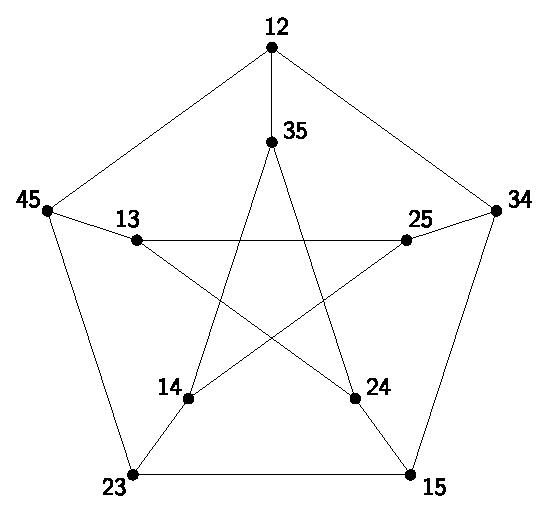
\includegraphics{images/petersen}
  \caption{Der Petersen Graph}
  \label{fig:petersen}
\end{figure}
Kneser gibt in \cite{Kneser55} eine obere Schranke f"ur die chromatische Zahl der Kneser Graphen an. Sp"ater zeigte Lov\'asz \todo{Referenz}, dass diese Schranke immer angenommen wird.
\begin{theorem}
  Ist $p\geq 2r-1$, so gilt
  $$\chi(K_{p:r}) \leq p-2r+2$$ \label{thm:kneserfarbung}
\end{theorem}
Der folgende Satz ist als Satz von Erd\H{o}s-Ko-Rado \cite{ErdosKoRado61} bekannt und gibt die Unabh"angigkeitszahl eines Kneser Graphen an.
\begin{theorem}
  Ist $p\geq 2r$ und $r \geq 2$, so gilt: 
  $$\alpha(K_{p:r})= \binom{p-1}{r-1}.$$
  \label{thm:ErdosKoRado}
\end{theorem}
Mit den beiden vorangegangenen S"atzen k"onnen wir nun beweisen, dass Kneser Graphen die Vermutung \ref{con:maincon} erf"ullen.
\begin{proposition}
  Seien $p\geq 2r-1$, $r\geq 1$ und sei $G= K_{p:r}$ ein Kneser Graph. Dann gilt $\chi(G) \leq \xi_{2}(G)$. 
\end{proposition}
\begin{proof}
  Sei $\chi(G) = k$. Wir machen eine Fallunterscheidung bez"uglich $r$.

  \ncase{1} {$r=1$} Dann ist $G=K_{p:1}$ isomorph zu $K_p$. Die Eigenwerte des $K_p$ sind alle gr"o{\ss}er als $-2$, insbesondere also auch $\lambda_{k}(G)$. Folglich ist $\chi(G) \leq \xi_{2}(G)$. 

  \ncase{2} {$p > 2r \geq 4 $} Sei $q = \alpha(G)$.  Dann ist nach Satz \ref{thm:ErdosKoRado} $ q = \binom{p-1}{r-1}$ und folglich $ q \geq p-1$. Nach Satz \ref{thm:kneserfarbung} ist $\chi(G) = p-2r+2 < p-2$. Folglich ist $q > \chi(G)$. 
  Dann gilt $$\chi(G) < q = \alpha(G) \leq \xi_{2}(G) $$ wegen Lemma \ref{lem:xieigenschaften}.

  \ncase{3} {$ p = 2r $} Die Ecken von $G$ sind alle $r$-elementingen Teilmengen von $\left\{ 1,\dots,p \right\}$. Da $p=2r$ ist f"ur ein $w\in V(G)$ die einzige benachbarte Ecke ihr Komplement in $\left\{ 1,\dots,p \right\}$. Also sind die Komponenten von $G$ alle isomorph zu $K_{2}$. Dann ist $\chi(G) = 2$ und $\omega(G) = 2$. 
  Aus Lemma \ref{lem:xieigenschaften} folgt dann $\xi_{2}(G) \geq \omega(G) = \chi(G)$.

  \ncase{4}{$k=2r+1$} Dann ist $|E(G)| = 0$ und folglich ist $G$ ein kantenloser Graph. Also ist $\alpha(G) = |G|$ und wir erhalten aus Lemma \ref{lem:xieigenschaften}, dass $\xi_{2}(G) \geq \alpha(G)$ gilt.
\end{proof}
Eine weitere Klasse die Vermutung \ref{con:maincon} erf"ullt, ist die Klasse der perfekten Graphen.

\begin{proposition}
  Sei $G$ ein perfekter Graph. Dann gilt 
  $\chi(G) \leq \xi_{2}(G)$.
\end{proposition}

\begin{proof}
  Da $G$ ein perfekter Graph ist, gilt $\chi(G) = \omega(G)$. 
  Mit Lemma \ref{lem:xieigenschaften} folgt dann $\xi_2(G) \geq \omega(G) = \chi(G)$.
\end{proof}

Planare Graphen sind nach dem Vierfarbensatz \todo{referenz} mit $4$ Farben f"arbbar. Der nachfolgende Satz garantiert, dass alle planaren Graphen der Ordnung mindestens $7$ Vermutung \ref{con:maincon} ebenfalls erf"ullen.
\begin{proposition}
  Sei $G$ ein planarer Graph mit $|G| \geq 7$. Dann gilt $\xi_{2}(G) \geq 4$.
  \label{prop:planaregraphen}
\end{proposition}

\begin{proof}
  Wir zeigen, dass $\lambda_4(G) > -2$ gilt. Dann ist $\xi_{2}(G) \geq 4$. 
  Nehmen wir daf"ur an, dass $\lambda_{4}(G) < -2$ gilt.
  Dann ist $\xi_{2}(G)\leq 3$. Aus Satz \ref{thm:xikantenschranke} folgt, dass f"ur die Zahl der Kanten $m$ von $G$ gilt:
  $$2m \geq \frac{4n(n-3)}{3}.$$
  Da $G$ ein planarer Graph ist, gilt zus"atzlich $$ m \leq 3n-6.$$
  Wir erhalten nun durch Umstellen die quadratische Ungleichung $$-2n^{2} +15n -18 \geq 0.$$
  L"osen dieser Ungleichung ergibt $ \frac{3}{2} \leq n \leq 6$, ein Widerspruch zur Vorrausetzung $n\geq 7$.
\end{proof} 
Aus dem vorhergehenden Satz erhalten wir sofort, dass jeder planare Graph die Vermutung \ref{con:maincon} erf"ullt.
\begin{corollary}
  Sei $G$ ein planarer Graph. Dann gilt $\chi(G) \leq \xi_{2}(G) $. 
\end{corollary}
\begin{proof}
  Die Aussage gilt offensichtlich f"ur den leeren Graph, also k"onnen wir annehmen, dass $G$ mindestens eine Ecke besitzt.
  Wir machen eine Fallunterscheidung bez"uglich der chromatischen Zahl $\chi(G)=k$. Auf Grund des $4$-Farbensatzes reicht es dann die F"alle $k=1,2,3,4$ zu betrachten.

  \ncase{1}{k = 1} Dann besitzt $G$ keine Kanten und mindestens eine Ecke. Deswegen besitzt $G$ nur den Eigenwert $\lambda_i = 0$ f"ur $1 \leq i \leq |G|$. Also ist $\xi_{2}(G) = |G| \geq 1$.

  \ncase{2}{k = 2} Dann ist $G$ bipartit und enth"alt mindestens eine Kante. Insbesondere ist $\omega(G) = 2$ und wir finden wegen Lemma \ref{lem:xieigenschaften} $\xi_{2}(G) \geq \omega(G) = 2 = \chi(G)$.

  \ncase{3}{k = 3} Ist $|G| \geq 7$, so ist wegen Satz \ref{prop:planaregraphen} nichts zu zeigen. Also reicht es den Fall $|G| \leq 6$ zu betrachten. Da $G$ nicht bipartit ist, besitzt $G$ nach dem Satz von K"onig einen ungeraden Kreis $C$ als Untergraphen. Da $|G| \leq 6$ gilt dann $|C| = 3$ oder  $|C| = 5$.
  Ist $|C| = 3$, so ist $\omega(G) \geq 3$ und die Behauptung folgt mit Lemma \ref{lem:xieigenschaften}. 
  Andernfalls ist $|C| = 5$ und wir k"onnen annehmen, dass $G$ dreiecksfrei ist. Wir zeigen, dass $C$ ein induzierter Untergraph von $G$ ist. Sei $C' = G[V(C)]$. Es bleibt zu zeigen, dass $E(C') = E(C)$ ist. Sei $uv\in E(C')\setminus E(C)$ eine Kante von $C'$, welche nicht in $C$ vorkommt. 
  Da $C$ ein Kreis der L"ange $5$ ist, besitzt $C$ den Durchmesser $2$. Da die Kante $uv$ nicht zu $C$ geh"ort, ist dann der Abstand zwischen $u$ und $v$ in $C$ gleich $2$. 
  Dann gibt es aber eine Ecke $w$ die in $C$ sowohl mit $u$ als auch mit $v$ benachbart ist.
  Deswegen ist $G[\{u,v,w\}]$ ein Kreis, im Widerspruch zu der Annahme, das $G$ dreiecksfrei ist.
  Deswegen ist $C$ ein induzierter Untergraph und wir finden wegen Beispiel \ref{ex:kreiseeigenwerte}:
  $$\xi_{2}(G) \geq \xi_{2}(C) = 5 > 3 = \chi(G).$$

  \ncase{4}{k = 4} $G$ enth"alt nach Satz \ref{thm:forbiddencritgraph} einen $4$-kritischen Untergraphen $G'$. Ist $|G'| \geq 7$, so ist wegen Satz \ref{prop:planaregraphen} $\xi_{2}(G') \geq 4$. Mit Lemma \ref{lem:xieigenschaften} folgt dann $\xi_{2}(G) \geq \xi_{2}(G') \geq 4 = \chi(G)$.
  Ist $|G'| \leq 6$, so folgt aus einem Resultat von Toft \cite{Toft74b}, dass $G' = K_4$ oder $G'$ den Kreis $C_5$ als induzierten Untergraphen enth"alt. Nun folgt $\xi_{2}(G) \geq \xi_{2}(G') \geq 4 = \chi(G)$. 

  Damit ist alles gezeigt.
\end{proof}

Berge \cite[Kapitel 15, Satz 2]{Berge91} zeigte, dass ein Graph $G$ der Ordnung $n$ und sein Komplement $\overline{G}$ stets die Ungleichung $\chi(G) + \chi(\overline{G}) \leq n+1$ erf"ullen. Au{\ss}erdem bewies Finck \cite{Finck66}, dass Gleichheit in dieser Ungleichung genau dann gilt, wenn $G$ von einem der beiden Graphentypen $F_1$ oder $F_2$ ist. 
Diese sind wie folgt definiert:
\todo{bessere formulierung}
Seien $n,p$ zwei nat"urliche Zahlen. Ein Graph $G$ geh"ort zum Typ $F_1 (n,p)$, falls $G$ aus einer unabh"angigen Menge $O$ der Ordnung $p$ und einem vollst"andigen Graphen $K$ der Ordnung $n-p+1$ besteht und es genau eine Ecke gibt, welche sowohl in $O$ als auch in $K$ vorkommt. Zwischen $O$ und $K$ d"urfen Kanten verlaufen. 

Ein Graph $G$ geh"ort zum Typ $F_2(n,p)$, falls $G$ aus einem Kreis $C=C_5$, einem vollst"andigen Graphen $K=K_{n-p-5}$ und einer unabh"angigen Menge $O=O_{p}$ besteht. 
Seien $v\in V(C), w\in V(K), u\in V(O)$ beliebig. Dann ist $vw\in E(G), vu\notin E(G) $ und $uw$ kann, muss aber nicht zu $E(G)$ geh"oren.

\begin{theorem}
  Sei $G$ ein Graph der Ordnung $n$. Dann gilt 
  $\xi_{2}(G) + \xi_{2}(\overline{G}) \geq n.$ 
  \label{thm:xikomplement}
\end{theorem}
\begin{proof}
  Seien $\xi_{2}(G) = l$, $A= A(G)$ die Adjazenzmatrix von $G$ und $\overline A = J-I-A = A(\overline{G})$ die Adjazenzmatrix von $\overline{G}$. 
  Ist $l = n$, so ist nichts zu zeigen. Wir betrachten also den Fall $l< n$. Dann ist $\lambda_{l+1}(A) \leq -2$. Zeigen wir $\xi_{2}(\overline{G}) \geq n-l$, so ist die Behauptung bewiesen. 
  Nach Satz \ref{thm:CourantFischer} ist 
  $$\lambda_{n-l}(\overline{A}) = \max\set{\min\limits_{x\in V , x \neq 0} R_{\overline{A}}(x)}{ V\subseteq \R^n \text{ linearer Unterraum,} \operatorname{dim}(V) =  n-l}.$$
  Ist also $V$ ein linearer Unterraum des $\R^{n}$ der Dimension $n-l$, so gilt $$\lambda_{n-l} (\overline{A}) \geq \min\limits_{x\in V, x\neq 0} R_{\overline{A}(x)}.$$
  Au{\ss}erdem folgt aus Satz \ref{thm:CourantFischer}, dass es einen linearen Unterraum $V$ des $\R^{n}$ der Dimension $n-l$ gibt mit $ \max \limits_{x\in V}R_{A}(x) =\lambda_{l+1} (A)  \leq -2$.
  Insbesondere ist also $R_{A}(x) \leq -2$ f"ur alle $x\in V$.
  Wir betrachten den Rayleigh Quotienten von $\overline{A}$ auf diesem Unterraum. Da $J$ positiv semidefinit ist, gilt f"ur alle $x\in V$ mit $x\neq 0$
  $$R_{\overline{A}}(x) = R_{J}(x) - R_I(x) - R_A(x) \geq  R_J(x) - 1 + 2 = R_J(x) +1  \geq 1.$$
  Dann ist $\lambda_{n-l}(\overline{A}) \geq \min\limits_{x\in V} R_{\overline{A}}(x) \geq 1$. 
  Also ist $\xi_{2}(\overline{G}) \geq n-l$. 
\end{proof}



\begin{theorem}
  Sei $G$ ein Graph. Dann gilt $\chi(G) + \chi(\overline{G}) \leq \xi_{2}(G) +  \xi_{2}(\overline{G})$.
  \label{thm:xichromatisch}
\end{theorem}
\begin{proof}
  Gilt $\chi(G) + \chi(\overline{G}) \leq n$, so ist nach Satz \ref{thm:xikomplement} nichts mehr zu zeigen. Andernfalls ist $G$ entweder vom Typ $F_1$ oder $F_2$. 

  \ncase{1}{$G$ ist vom Typ $F_1(n,p)$} Dann ist $\omega(G) = n-p+1$ und $\omega (\overline{G})=p$. Dann folgt mit Lemma \ref{lem:xieigenschaften}, dass 
  $$\xi_{2}(G) + \xi_{2}(\overline{G}) \geq \omega(G) + \omega(\overline{G}) = n+ 1 = \chi(G) + \chi(\overline{G}).$$

  \ncase{2}{$G$ ist vom Typ $F_2(n,p)$} Wir betrachten den induzierten Untergraphen $H=G[V(C) \cup V(O)]$. Dann ist $H$ die disjunkte Vereinigung eines kantenlosen Graphen und eines $C_5$. Es gilt $|H| = p+5$ und aus Beispiel \ref{ex:disjointunion} sowie Beispiel \ref{ex:kreiseeigenwerte} folgt, dass $\xi_{2}(H) = |H|$. 
  F"ur $\tilde{H} = \overline{G} (V(C) \cup V(K))$ gilt dann nach dem selben Argument $$\xi_{2}(\tilde{H}) = |\tilde{H}| = |V(C)| + |V(K)| = n-p .$$ Dann gilt 
  $$\xi_{2}(G) + \xi_{2}(\overline{G}) \geq \xi_{2}(H) + \xi_{2}(\overline{H}) = p+5 + n -p = n+ 5 > n+ 1 = \chi(G) + \chi(\overline{G}).$$
  Damit ist alles gezeigt.
\end{proof}

\begin{corollary}
  Sei $G$ ein Graph. Dann gilt mindestens eine der folgenden Aussagen:
  \begin{enumerate}[label=\rm{(\alph*)}]
    \item $\xi_2(G) \geq \chi(G)$.
    \item $\xi_{2}(\overline{G}) \geq \chi(\overline{G})$.
  \end{enumerate}
\end{corollary}

\begin{proof}
  Angenommen, beide Aussagen gelten nicht. Dann ist 
  $$\xi_2(G) + \xi_{2}(\overline{G}) < \chi(G) + \chi(\overline{G}), $$
  im Widerspruch zu Satz \ref{thm:xichromatisch}.
\end{proof}

